\documentclass[11pt]{article}
\usepackage[left=1in, right=1in, top=0.75in, bottom=1in]{geometry}
\usepackage{mathexam}
\usepackage{amsmath}
\usepackage{graphicx}
\usepackage[export]{adjustbox} %positioning of images
\usepackage[dvipsnames]{xcolor}
\usepackage{enumitem}
\usepackage{setspace}
\usepackage{latexsym}
\usepackage{wasysym}
\usepackage{amssymb}
\usepackage{pgfplots}
\usepackage{comment}
\usepackage{exsheets}
\usepackage{pdfpages}
\usepackage{multicol}

\ExamClass{Math 242}
\ExamName{Classwork }
\ExamHead{Fall 2024}
\fancyfoot{}
\setlength{\headheight}{13.59999pt}

\let\ds\displaystyle
\newcommand{\ddx}{\frac{d}{dx}}
\newcommand{\red}{\textcolor{red}}
\newcommand{\blue}{\textcolor{blue}}
\newcommand{\pink}{\textcolor{CarnationPink}}
\newcommand{\orange}{\textcolor{orange}}
\newcommand{\purple}{\textcolor{purple}}
\newcommand{\violet}{\textcolor{violet}}
\newcommand{\cyan}{\textcolor{cyan}}
\newcommand{\grn}{\textcolor{green}}
\newcommand{\uh}{\textcolor{ForestGreen}}
\newcommand{\bas}[1]{\begin{align*}{#1}\end{align*}}

\pgfplotsset{compat=1.18}

\pgfplotsset%Default tikz axis style
{
    axis lines=center, 
    grid,
    grid style={very thin, densely dotted, black!50},
    xmin=-5,    xmax=5,         xtick distance=1,
    ymin=-5,    ymax=5,         ytick distance=1,
    restrict y to domain=-10:10, % <-------
    ticklabel style={font=\scriptsize, fill=white, inner sep=2pt},
    domain=-5:5, samples=100,
    no marks, 
    every axis plot post/.append style={ultra thick, semitransparent,},
}

\pgfkeys{/pgfplots/Axis Style/.style=
{
    grid style={thin, densely dotted, black!50},
    width=11.5cm, height=5cm,
    axis x line=center, 
    axis y line=middle, 
    samples=100,
    ymin=-1.1, ymax=1.1,
    xmin=-.1, xmax=6.4,
    domain=0:2*pi
}}

\def\myalign#1{%
  \def\trule{\noalign{\smallskip\hrule\medskip}}
  \def\nebc{\nearrow\bigcup}
  \def\sebc{\searrow\bigcup}
  \def\pminf{{}_{-\infty}|^{+\infty}}
  \let\Inf\infty
  \def\amp{&}% props to Bruno; I just love this trick
  \vbox{\mathsurround0pt\openup1\jot
    \halign{%
      &$\displaystyle##\hfil\tabskip0pt$&\amp##\tabskip1em\crcr
      \noalign{\hrule height1pt\smallskip}#1\noalign{\smallskip\hrule height1pt}\crcr}}}

\linespread{1.3}

\begin{document}

    \hrule
    \vspace{.5cm}
    \noindent\textbf{Name:} \underline{\qquad\qquad\qquad\qquad\qquad\qquad\qquad\qquad\qquad\qquad\qquad\qquad\qquad}

    Alright, so I think this was the problem we were looking at. Here's the way where we take the coefficient out
    \bas
    {
        \int\frac{\frac{5}{6}}{x+2}dx   &=  \frac{5}{6}\int\frac{1}{x+2}dx\\[1em]
                                        &=  \frac{5}{6}\ln|x+2|+c.
    }

    \bas
    {
        \int\frac{\frac{5}{6}}{x+2}dx   &=  5\int\frac{1}{6(x+2)}dx\\[1em]
                                        &=  5\int\frac{1}{6x+12}dx\\[1em]
    }
    Use $u$-substitution with $u=6x+12$, $du=6dx$, so $dx=\frac{1}{6}du$ and we get

    \bas
    {
         5\int\frac{1}{6x+12}dx &=  5\int\frac{\frac{1}{6}}{u}du\\[1em]
                                &=  \frac{5}{6}\int\frac{1}{u}du\\[1em]
                                &=  \frac{5}{6}\ln|u|+c\\[1em]
                                &=  \frac{5}{6}\ln|6x+12|+c.
    }

    So it really does seem like something weird is going on, but we can rewrite this as

    $$\frac{5}{6}\ln|x+2|+\frac{5}{6}\ln(6)+c.$$

    The thing is, $c$ doesn't have a set value, and $\frac{5}{6}\ln(6)$ is just a number, so $\frac{5}{6}\ln(6)+c$ can just be called a new constant, $k$, giving us that our answer is 
    $$\frac{5}{6}\ln|x+2|+k.$$

    Our mistake was forgetting that when we take a derivative we lose some information that can never be gotten back, namely the height of the function. The integral tells us the shape of the function we differentiated, but not it's vertical position, so it's not that $$\frac{5}{6}\ln|x+2|=\frac{5}{6}\ln|6x+2|,$$
    it's simply that the two functions have the same shape, one is just further away from the $x$-axis than the other. We can see that by looking at the graphs of the two functions. The red graph is of $\frac{5}{6}\ln|x+2|$ and the blue is of $\frac{5}{6}\ln|6x+12|$.
    \begin{center}
        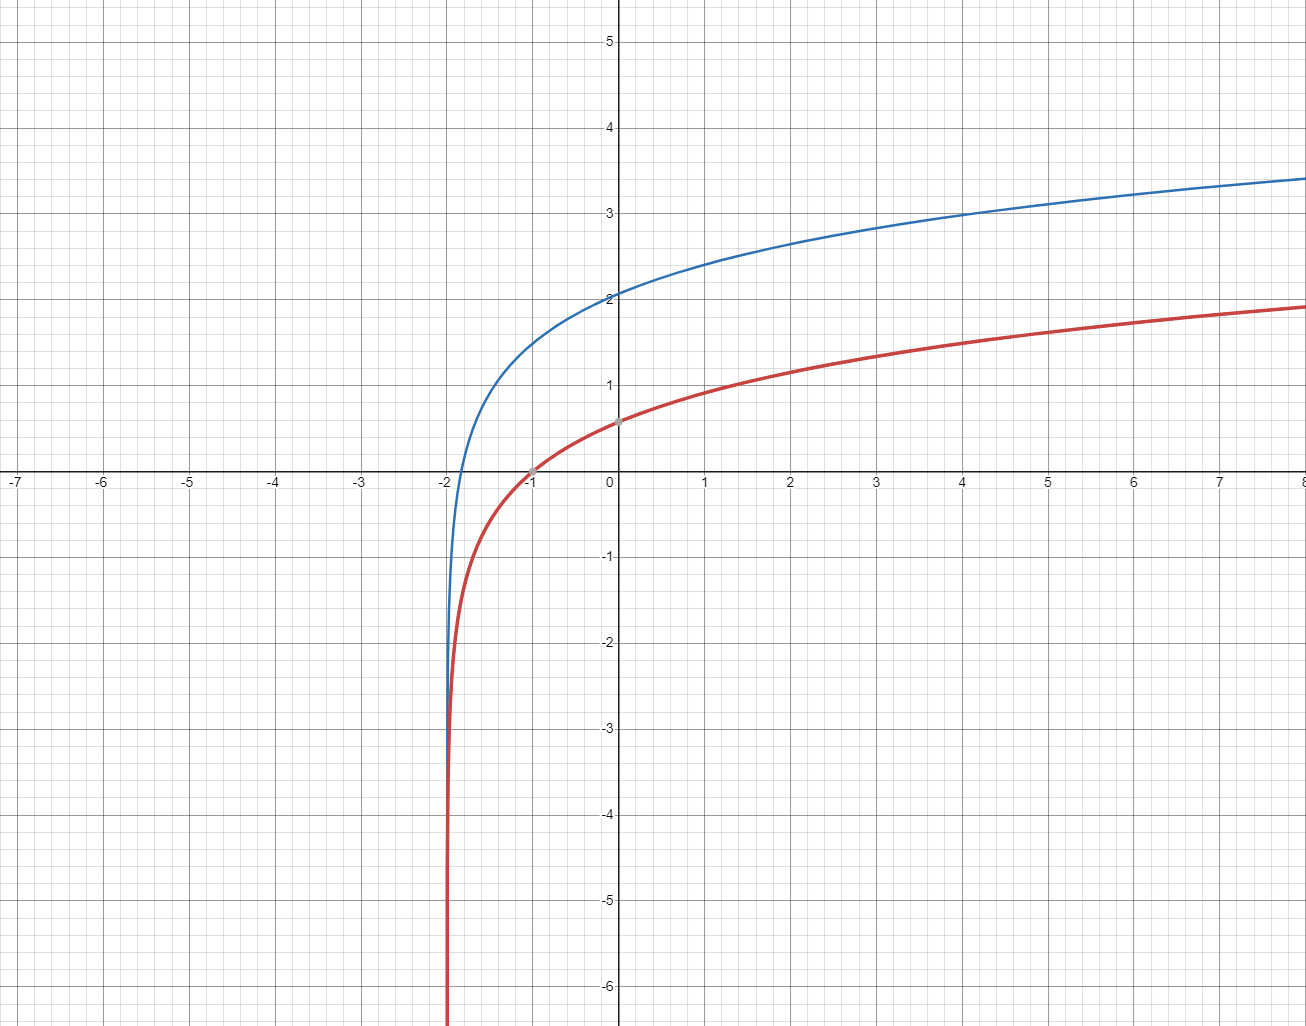
\includegraphics[width=16cm]{F24/Misc. Notes/Halvor-notes.png}
    \end{center}
\end{document}